\documentclass{standalone}
\usepackage{tikz}
\usetikzlibrary{shapes,arrows}

\tikzstyle{block} = [rectangle, draw, 
    text width=3em, text centered, minimum height=3em]
\tikzstyle{round} = [circle, draw, 
    text width=3em, text centered, minimum height=3em]

\begin{document}
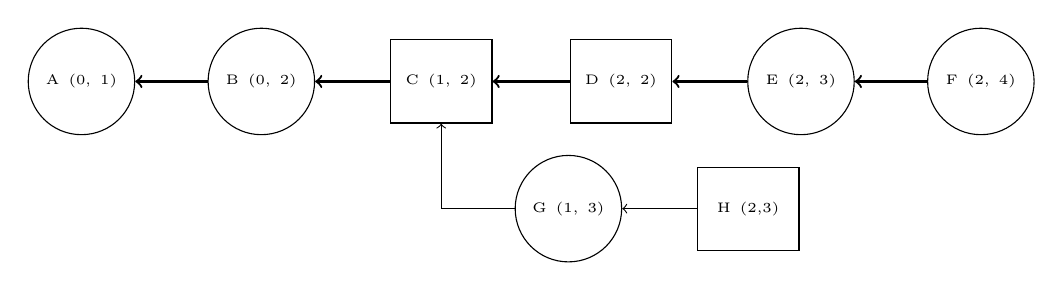
\begin{tikzpicture}[node distance = 6.5em, auto]
    \node (b1) [round] {\tiny A (0, 1)};
    \node (b2) [round, right of=b1] {\tiny B (0, 2)};
    \node (b3) [block, right of=b2] {\tiny C (1, 2)};
    \node (b4) [block, right of=b3] {\tiny D (2, 2)};
    \node (b5) [round, right of=b4] {\tiny E (2, 3)};
    \node (b6) [round, right of=b5] {\tiny F (2, 4)};
    
    % new branch bottom
    \node (c1) [round, below right of= b3] {\tiny G (1, 3)};
    \node (c2) [block, right of= c1] {\tiny H (2,3)};

    \draw [<-, thick] (b1) -- (b2);
    \draw [<-, thick] (b2) -- (b3);
    \draw [<-, thick] (b3) -- (b4);
    \draw [<-, thick] (b4) -- (b5);
    \draw [<-, thick] (b5) -- (b6);
    
    \draw [<-] (b3) |- (c1);
    \draw [<-] (c1) -- (c2);
    
    % these are lines references PoS
    % \draw [line, dashed] (b5) |- ([yshift=-0.75em]b2.south) |- (b2.south);
    % \draw [line, dashed] (c2) |- ([yshift=-0.75em, xshift=-12em]c2.south) |- (b3.south west);
\end{tikzpicture}
\end{document}